\section{Data Governance and Management}
As we have said countless times up to this point, cloud computing is a very complex matter, the NIST definition can be found back in section 5.4 and the issues of the model are the following:
\begin{itemize}
    \item (Micro)Services composition
    \item Untrustworthy data
    \item High dynamics and flexibility
    \item Multi-domain evaluation
\end{itemize}
The natural evolution of cloud spanning an even bigger area is IoT, IoT is \textit{The intelligent connectivity of physical devices driving massive gains in efficency, business growth and quality of life}. \n
The first big step in that direction was made with 5G, high-speed connectivity with very low latency is one of the basic requirements to start setting up the needed infrastructure for a smart city. \n
In an IoT setting the cloud will have a layered and hierarchical structure with cloud data centers, that exchange informations with fog nodes that pre-process data coming from the edge of the cloud which are all the cameras and sensors embedded in smart systems. Having many sensors connected and collecting data every minute requires a very good metrics and analytics system to process the data coming from the edge and implement specific management functionalities. \n
It's obvious that the time has come to talk a bit about big data and more data driven techniques. \n
The 5 Vs of big data are the following:
\begin{itemize}
    \item Volume, the size of the data
    \item Velocity, the speed at which the data is generated
    \item Variety, the different types of data
    \item Veracity, The trustworthiness of the data in terms of accuracy
    \item Value, having data is of no use unless they can be turned into value
\end{itemize}
The data analytics pipeline is shown in figure 12
\begin{figure}
    \centering
    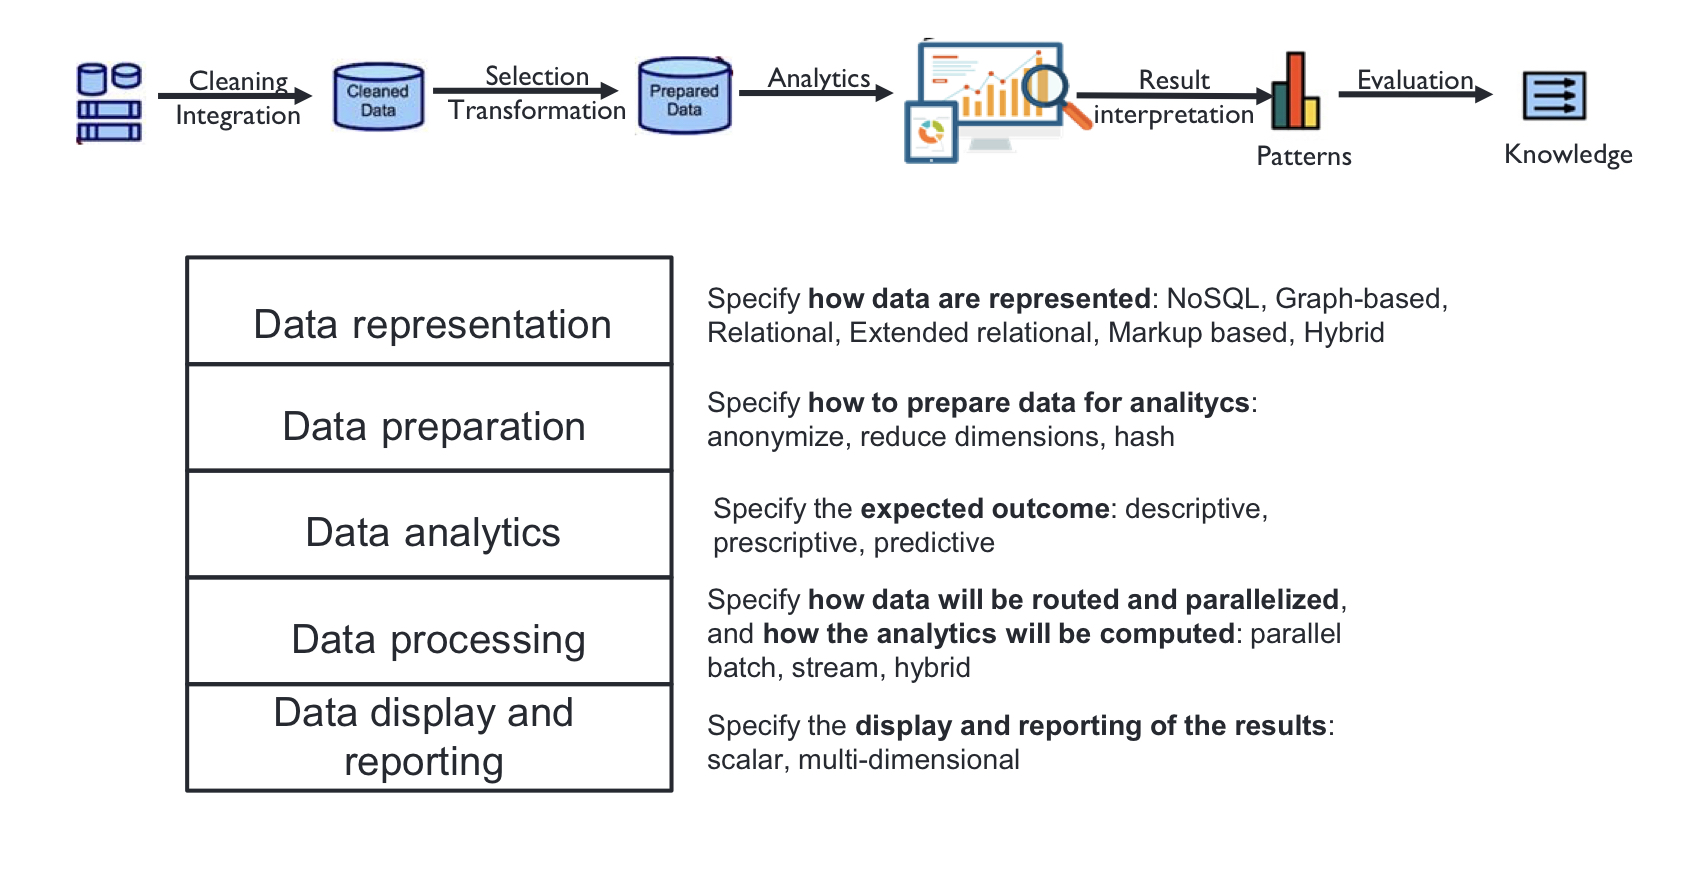
\includegraphics[scale=0.2]{Images/data_analytics_pipeline.jpeg}
    \caption{The data analytics pipeline}
\end{figure}
Since companies have seen how profitable can be a data-driven development process big data technologies have grown tremendousl in the past few years but there has been an incredible shortage of data scientists and data engineers, the demand is far from being met. \n
Only 30\% of businesses have a fully integrated data-analytics pipeline, 38\% of the businesses are struggling even with proofs of concept, key challenges associated with the development and management of Big Data initiatives are:
\begin{itemize}
    \item Lack of skills and clarity on Big Data technology (many people in the business do not even know that in data there is money to be made)
    \item Lack of general architecture and lack of standard processes
    \item Ineffective governance models
\end{itemize}
The biggest implementation challenges today in the field of Big Data are that: it's really hard to store and manage data in different places and formats, plus there is no coordintation in the field of big data / AI initiatives, solving the problem of handling massive amounts of data is not trivial both from an implementation and an engineering stand point, dated data and inability to operationalize insights and big data tool selection. \n
Getting into big data at this point in time can be done with many open source alternatives when it comes to both big data processing frameworks, storage and implementation languages. The incredible amount of alternatives allows companies to choose whichever technological stack they prefer without having to bind to one specific producer. \n
As I said, thanks to the power of alternatives, there are a bunch of commercial analytics platforms that are built on top of big data open source technologies (Apache Hadoop, Spark, Storm, etc...) the leaders in this space are Cloudera, Hortonworks and IBM insights, this is a summary of their features:
\begin{itemize}
    \item Provide enterprise-ready Hadoop distributions
    \item Management of Hadoop clusters
    \item Performance analytics
    \item Security and SLA monitoring
    \item Support for integrated marketing solutions
\end{itemize}
When it comes to data governance most technologies also offer data preparation functionalities like: ETL or ELT (Extract, Transform and Load). \n
Data storage and preparation tools offer:
\begin{itemize}
    \item Data inventory
    \item Metadata management
    \item Data quality
    \item Data integration
    \item Data security
    \item Fault tolerance
    \item ELT, ETL
    \item SLA monitoring
\end{itemize}
There are many providers when it comes to analytics and visualization technology. A summary of the offered features is:
\begin{itemize}
    \item Graphical interface to design analytics model
    \item Store the analysis result to different databases
    \item Provide data training and validation environment
\end{itemize}
Up to this moment we have basically reinforced the fact that there is a plethora of different big data technologies to choose from, picking a stack that suits the needs of the client can be a very complex task, it's important to keep in mind the fact that there is no single big data technology and balance between bottom-up and top-down approaches should be found. An example of the selection process is shown in figure 13.
\begin{figure}
    \centering
    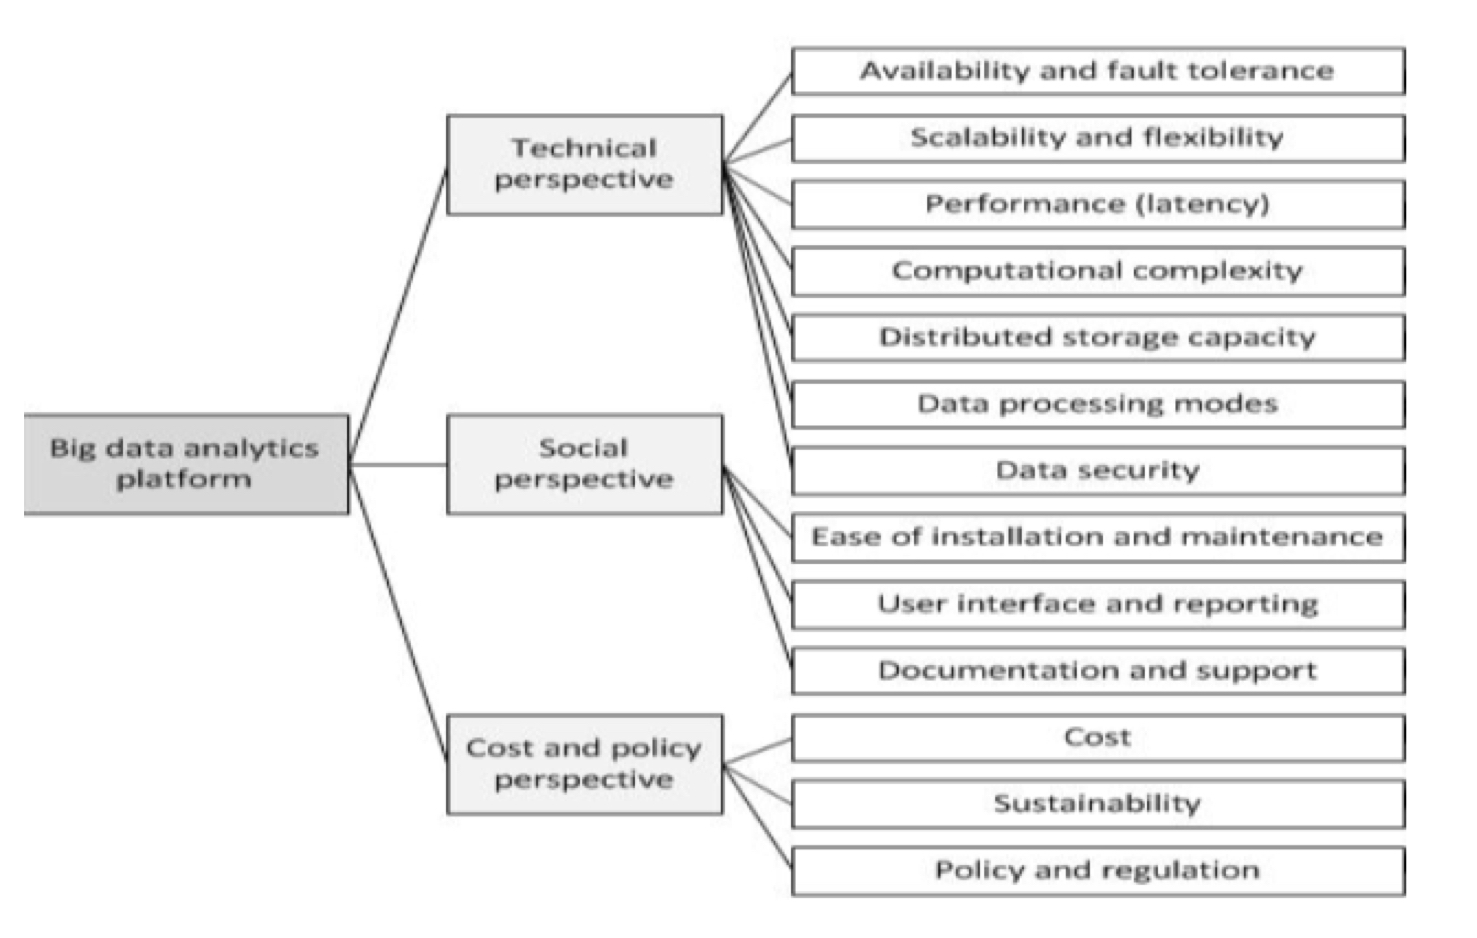
\includegraphics[scale=0.2]{Images/tech_selection_process.jpeg}
    \caption{Example of criterion to select big data technologies}
\end{figure}
\subsection{Big Data as a Service (BDaaS)}
We have said that entering the world of big data is a hustle, we have also said that there are not enough people to meet the work demand in the field and that there is a heck of a lot of money to be made from the good use of users data. \n
Point is? \n
A new company wanting to enter the scene (not necessarily in the tech world) and needing a big data system gets to a point where they find themselves in a situation where they have options, too many options, and no easy solution to all the mess. \n
Somebody thought it would be really cool to merge cloud business logic with big data. What if, I gave you a ready to use infrastructure, no further knowledge required, to handle your big data needs, in exchange for a fee? No need to lose your wits on a big data infrastructure implementation, that's for sure. \n
BSaaS are not just about storage and cost, these solutions offer built-in systems for artificial intelligence and analytics, you can accomplish some pretty impressive results without having to have a huge team of data analysts, scientists and architects around you. \n
The advantages of BDaaS are pretty obvious:
\begin{itemize}
    \item Makes managing big data easier
    \item Opens up big data for a range of medium-sized businesses
    \item It's a very low cost solution compared to the alternative of running your own metal (just like with the clud)
\end{itemize}
There are three different BDaaS models:
\begin{itemize}
    \item Big data infrastructure as a service, it's a IaaS offer including basic data services from a cloud serivce provider.
    \item Big data platform as a service, is a PaaS offer for an all-round big data stack.
    \item Big data software as a service, a SaaS offer which is self contained in a single tool.
\end{itemize}
How does the big data IaaS model work? There is a data layer, consisting of either: Hadoop, NoSequel databases and Relational databases; a compute layer, which can either be: Self-built ETL scripts, Commercial ETL tools or open source processing tools. \n
If we climb the stack a PaaS model can be (if we consider Amazon's implementation) a standard Hadoop implementation with:
\begin{itemize}
    \item Data ingestion, logs file data from any data source
    \item Amazon S3 data storage layer
    \item Analytics and visualization
\end{itemize}
A similar setup is implemented by competitors. \n
Last but not least, getting to the SaaS level, a fully hosted big data stack that includes everything from data storage to data visualization has the following:
\begin{itemize}
    \item Data layer
    \item Integration layer, pulls the data out of the database and into a flexible modeling layer
    \item Processing layer
    \item Analytics and BI layer
\end{itemize}
The differences between the various models can be summarized as follows:
\begin{itemize}
    \item IaaS is way more expensive than the other two models but allows almost complete control over resources and allows a custom implementation of complex data pipelines. It is not an easy thing to handle and is an hardcore alternative.
    \item PaaS is a much easier thing to master, it allows for a decent level of customization and control but it also requires a good level of expertise to handle compared to SaaS options.
    \item SaaS is a very low cost solution which is not that customizable but can tick many boxes for low to medium sized companies.
\end{itemize}